\subsection{Bases de Dados e Pré-processamento}

Neste trabalho, utilizamos os conjuntos \textbf{Adult} (Census Income) e \textbf{Dry Bean}, ambos amplamente empregados em tarefas de classificação e agrupamento. Para garantir comparabilidade, aplicou-se um pré-processamento padronizado: variáveis categóricas foram convertidas em numéricas, atributos normalizados e os dados divididos estratificadamente em 70\% para treino e 30\% para teste. Também foi realizado balanceamento por oversampling, igualando o número de exemplos em cada classe antes da divisão.

\textbf{Adult:} Aproximadamente 48 mil amostras de adultos dos EUA, com atributos demográficos e socioeconômicos, distribuídas em duas classes principais (renda $>$50K e $\leq$50K). O balanceamento foi essencial para evitar predominância de uma classe e garantir avaliações justas.

% Distribuição das classes - Adult
A Figura~\ref{fig:adult_freq_antes} apresenta a distribuição das classes no dataset Adult antes do balanceamento. Após o balanceamento, a nova distribuição pode ser observada na Figura~\ref{fig:adult_freq_depois}.

\begin{figure}[ht]
    \centering
    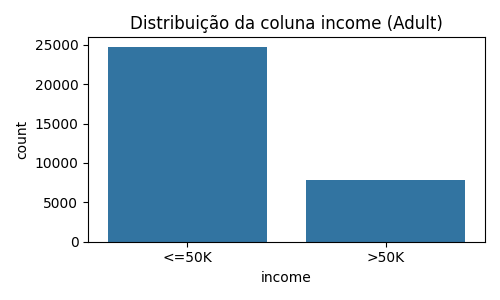
\includegraphics[width=0.7\linewidth]{../src/img/adult_income_hist_before_balance.png}
    \caption{Distribuição das classes no dataset Adult antes do balanceamento ($n=\sim48.842$ amostras).}
    \label{fig:adult_freq_antes}
\end{figure}

\begin{figure}[ht]
    \centering
    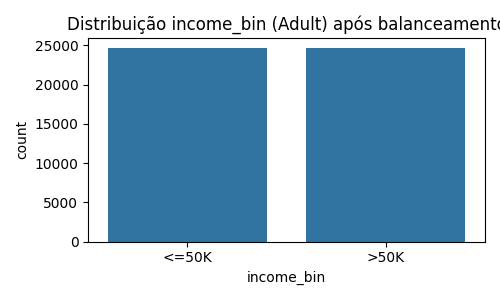
\includegraphics[width=0.7\linewidth]{../src/img/adult_income_hist_after_balance.png}
    \caption{Distribuição das classes no dataset Adult após o balanceamento por oversampling ($n=73.842$ amostras).}
    \label{fig:adult_freq_depois}
\end{figure}

\textbf{Dry Bean:} O conjunto Dry Bean possui 13.611 amostras de feijões secos, distribuídas em sete classes principais (cultivares): Seker, Barbunya, Bombay, Cali, Horoz, Sira e Dermason, com atributos morfológicos extraídos de imagens. Apesar de uma distribuição mais equilibrada que o Adult, algumas cultivares eram minoritárias, tornando o balanceamento importante para análises imparciais.

% Distribuição das classes - Dry Bean
A Figura~\ref{fig:drybean_freq_antes} mostra a distribuição das classes no dataset Dry Bean antes do balanceamento. A distribuição das classes após o balanceamento está ilustrada na Figura~\ref{fig:drybean_freq_depois}.

\begin{figure}[ht]
    \centering
    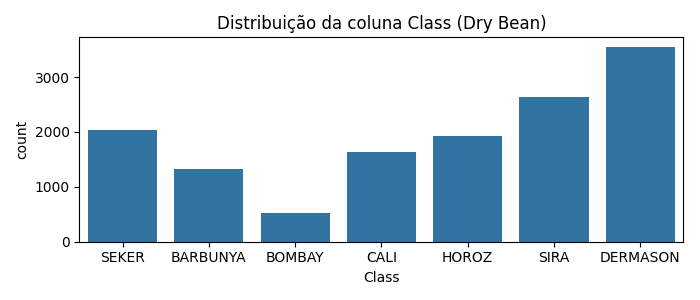
\includegraphics[width=0.7\linewidth]{../src/img/drybean_class_hist_before_balance.png}
    \caption{Distribuição das classes no dataset Dry Bean antes do balanceamento ($n=13.611$ amostras).}
    \label{fig:drybean_freq_antes}
\end{figure}

\begin{figure}[ht]
    \centering
    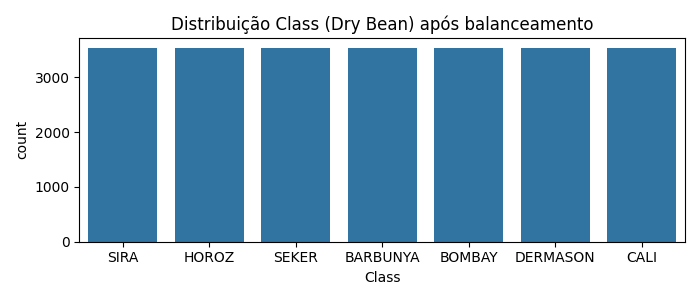
\includegraphics[width=0.7\linewidth]{../src/img/drybean_class_hist_after_balance.png}
    \caption{Distribuição das classes no dataset Dry Bean após o balanceamento por oversampling ($n=24.822$ amostras).}
    \label{fig:drybean_freq_depois}
\end{figure}

A Figura~\ref{fig:drybean_pca_true_labels} mostra a projeção das amostras do Dry Bean balanceado no espaço 2D do PCA, coloridas pelas classes verdadeiras, enquanto a Figura~\ref{fig:adult_pca_true_labels} apresenta a projeção das amostras do Adult balanceado, também coloridas pelas classes verdadeiras.

% Visualização PCA das classes verdadeiras - Dry Bean
\begin{figure}[ht]
    \centering
    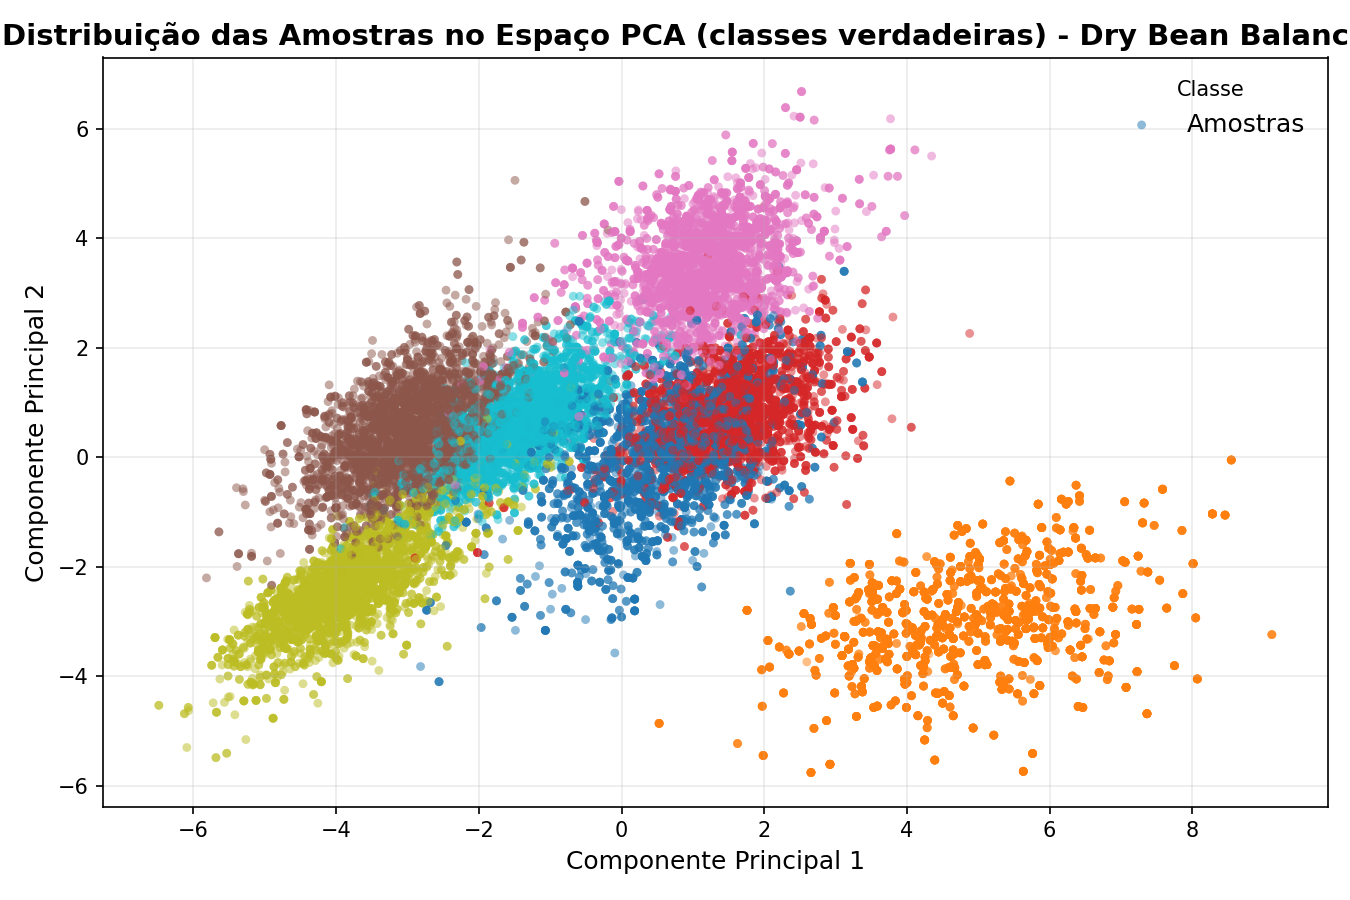
\includegraphics[width=0.8\linewidth]{../src/img/kmeans_drybean_balance_pca_true_labels.png}
    \caption{Projeção das amostras do Dry Bean balanceado no espaço 2D do PCA, coloridas pelas classes verdadeiras.}
    \label{fig:drybean_pca_true_labels}
\end{figure}

% Visualização PCA das amostras - Adult
\begin{figure}[ht]
    \centering
    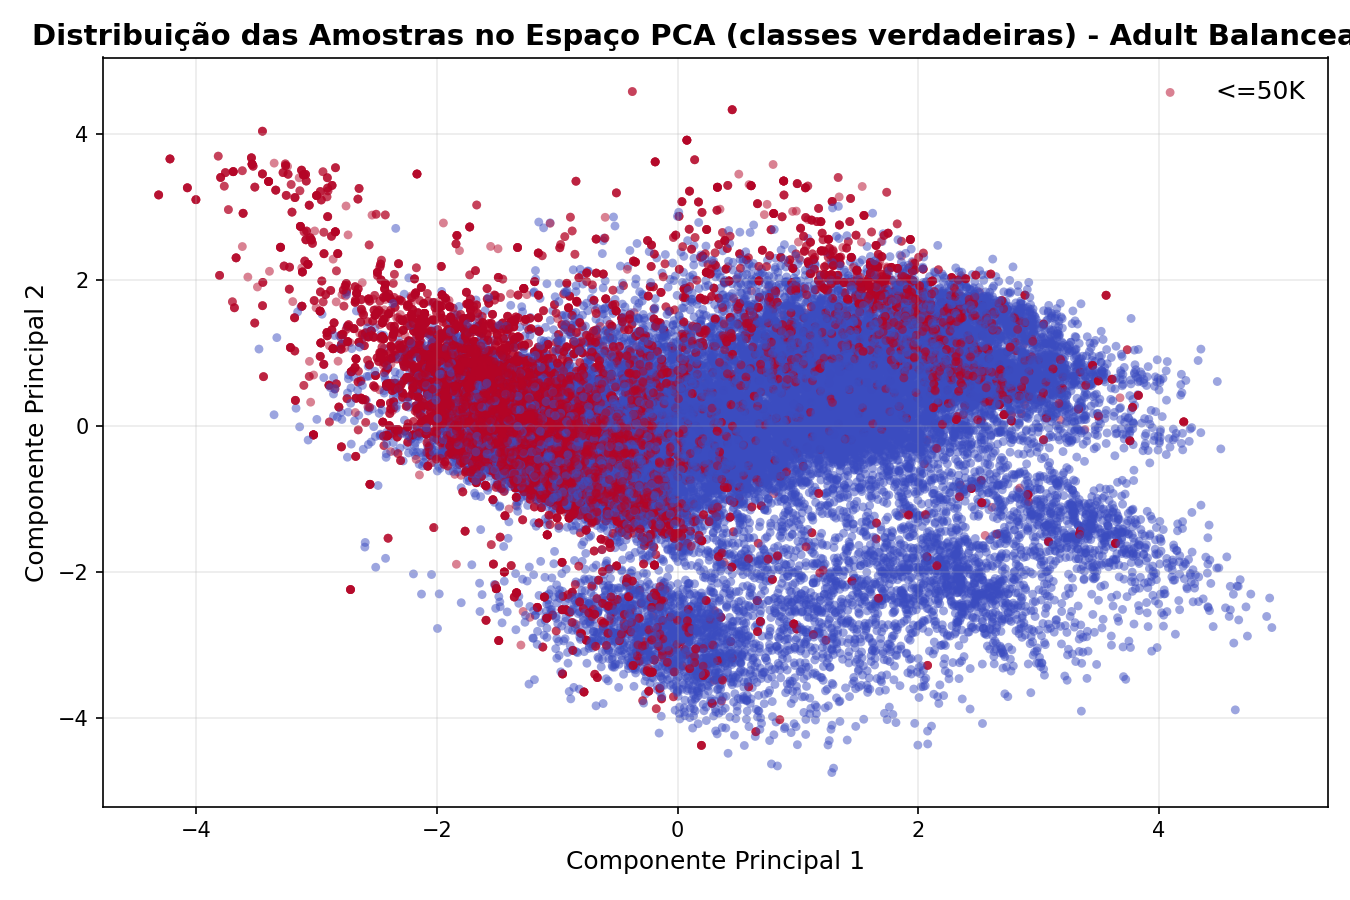
\includegraphics[width=0.8\linewidth]{../src/img/kmeans_adult_balance_pca_true_labels.png}
    \caption{Projeção das amostras do Adult balanceado no espaço 2D do PCA, coloridas pelas classes verdadeiras.}
    \label{fig:adult_pca_true_labels}
\end{figure}